% !TeX program = lualatex
% !BIB program = biber
% Auriga theme
% https://github.com/anishathalye/auriga

\documentclass[14pt,aspectratio=169]{beamer}
\usepackage{pgfpages}
\usepackage{fancyvrb}
\usepackage{ulem}
\usepackage{tikz}
\usepackage{multimedia}
\usepackage{media9}
\usepackage{minted}
\usetikzlibrary{positioning, chains,scopes,fit, backgrounds, shapes.misc, calc, patterns}
\usepackage{pgfplots}
\usepackage{pgfplotstable}
\usepackage{array}

\tikzset{ %
	invisible/.style={opacity=0}, %
	visible on/.style={alt={#1{}{invisible}}},%
	trans/.style={opacity=0.2},%
	trans on/.style={alt={#1{}{trans}}},%
	alt/.code args={<#1>#2#3}{%
		\alt<#1>{\pgfkeysalso{#2}}{\pgfkeysalso{#3}} % \pgfkeysalso doesn't change the path
	},%
}%a

% color blind friendly color scheme for qualitative data http://personal.sron.nl/~pault/
\definecolorset{RGB}{tol}{}{blue,68,119,170;cyan,102,204,238;green,34,136,51;yellow,204,187,68;red,238,102,119;purple,170,51,119;grey,187,187,187}

\pgfplotscreateplotcyclelist{bright}{%
	tolblue,every mark/.append style={fill=tolblue!80!black},mark=*\\%
	tolcyan,every mark/.append style={fill=tolcyan!80!black},mark=square*\\%
	tolgreen,every mark/.append style={fill=tolgreen!80!black},mark=triangle*\\%
	tolyellow,every mark/.append style={fill=tolyellow!80!black},mark=star\\%
	tolred,every mark/.append style={fill=tolred!80!black},mark=diamond*\\%
	tolpurple,every mark/.append style={solid,fill=tolpurple!80!black},mark=pentagon*\\%
	tolgrey,every mark/.append style={solid,fill=tolgrey!80!black},mark=10-pointed star\\%
}

\pgfplotsset{compat=1.18,%
	/pgfplots/bar  cycle  list/.style={/pgfplots/cycle  list={%
			{tolblue!20!black,fill=tolblue,mark=none},%
			{tolcyan!20!black,fill=tolcyan,mark=none},%
			{tolgreen!20!black,fill=tolgreen,mark=none},%
			{tolyellow!20!black,fill=tolyellow,mark=none},%
			{tolred!20!black,fill=tolred,mark=none},%
			{tolpurple!20!black,fill=tolpurple,mark=none},%
			{tolgrey!20!black,fill=tolgrey,mark=none},%
		}
	},
	cycle list name=bright,
	table/search path={../data},
}

\graphicspath{{imgs/}}

\ifnotes
\setbeamertemplate{note page}[plain]
\setbeameroption{show notes on second screen=right}
\fi

\usetheme{auriga}
\usecolortheme{auriga}

\usepackage[backend=biber, autocite=footnote, style=authortitle, maxcitenames=3]{biblatex}
\bibliography{library}
\usepackage{xpatch}
\xapptobibmacro{cite}{\setunit{\nametitledelim}\textcolor{gray}{\printfield{year}}}{}{}

\usepackage{listings}
\usepackage[capitalise]{cleveref}
\usepackage{amsfonts}
\usepackage{siunitx}

% footnotes are currently only used for citations
\setbeamerfont{footnote}{size=\scriptsize}

% define some colors for a consistent theme across slides
\definecolor{red}{RGB}{181, 23, 0}
\definecolor{blue}{RGB}{0, 118, 186}
\definecolor{gray}{RGB}{146, 146, 146}

\definecolor{commentcolor}{RGB}{0, 128, 0}

\newcommand{\R}{\mathbb{R}}

%\newcommand{\DB}[1]{{\color{blue!60!black}#1}}
%\newcommand{\DR}[1]{{\color{red!60!black}#1}}
%\newcommand{\DG}[1]{{\color{green!60!black}#1}}
\newcommand{\DB}[1]{{\color{tolblue}#1}}
\newcommand{\DR}[1]{{\color{tolred}#1}}
\newcommand{\DG}[1]{{\color{tolgreen}#1}}

\newcommand{\white}[1]{{\color{white}#1}}

\definecolor{color1}{RGB}{146, 146, 146}
\newcommand{\colorboxDR}[1]{\fboxsep0pt\colorbox{tolyellow!25}{#1}}
\newcommand{\colorboxDB}[1]{\fboxsep0pt\colorbox{tolblue!25}{#1}}
\newcommand{\highlightDR}[1]{{\alt<1-2>{#1}{\colorboxDR{$#1$}}}}
\newcommand{\highlightDB}[1]{{\alt<1-3>{#1}{\colorboxDB{$#1$}}}}
%\newcommand{\highlightListing1}[1]{\fboxsep0pt\colorbox{tolyellow!25}{\texttt{#1}}}
%\newcommand{\highlightListing2}[1]{\fboxsep0pt\colorbox{tolblue!25}{\texttt{#1}}}
%\newcommand{\highlightDR}[1]{{\alt<1>{#1}{\fboxsep0pt\colorbox{tolyellow!25}{$#1$}}}}
%\newcommand{\highlightDB}[1]{{\alt<1-2>{#1}{\fboxsep0pt\colorbox{tolblue!25}{$#1$}}}}

\newcommand{\mytikzmark}[1]{%
	\tikz[overlay,remember picture,baseline] \coordinate (#1) at (0,0) {};}
\newcommand{\highlight}[2]{%
	\draw[tolyellow,line width=10pt,opacity=0.25]%
	([yshift=3pt]#1) -- ([yshift=3pt]#2);%
}
\newcommand{\highlightAlt}[2]{%
	\draw[tolblue,line width=10pt,opacity=0.25]%
	([yshift=3pt]#1) -- ([yshift=3pt]#2);%
}
\newcommand{\highlightDummy}[2]{%
	\draw[tolyellow,line width=10pt,opacity=0.0]%
	([yshift=3pt]#1) -- ([yshift=3pt]#2);
}

\let\svthefootnote\thefootnote
\newcommand\blankfootnote[1]{%
	\let\thefootnote\relax\footnotetext{#1}%
	\let\thefootnote\svthefootnote%
}

%\newcommand{\highlight3}[1]{{\alt<1-3>{#1}{\colorbox{tolgray!50}{$#1$}}}}
\newcommand{\gray}[1]{{\color{gray}#1}}

\title{Introduction to PyTorch\\ {\normalsize Deep Learning for Scientific Computing}}

\author{Robert Jendersie}

%\institute[shortinst]{\inst{1} Otto-von-Guericke Universität Magdeburg \samelineand \inst{2} ECMWF Bonn}

\begin{document}

{
  % rather than use the frame options [noframenumbering,plain], we make the
  % color match, so that the indicated page numbers match PDF page numbers
  \setbeamercolor{page number in head/foot}{fg=black}
  \begin{frame}
    \titlepage
  \end{frame}
}

\section{Introduction}

	\tikzset{%
	Box/.style={minimum width=3cm, minimum height=2.cm, draw=black},
}

\begin{frame}{Ingredients}
	\centering
	\begin{tikzpicture}
		\node(problem)[Box, label=below:Problem]{
\includegraphics[height=0.8cm]{data.png} {\Huge $\rightarrow$} 
\includegraphics[height=0.8cm]{data.png}};
		\node(neuralNetwork)[Box,  trans on=<2->,  label={[trans on=<2->]below:Neural Network}, right= of problem]{\includegraphics[height=1.4cm]{neuralnet-symbol.pdf}};
		\node(optimizer)[Box,  label={[trans on=<3->]below:Optimizer}, trans on=<3->, right= of neuralNetwork]{{\Huge $\mathcal{L}$}}; % 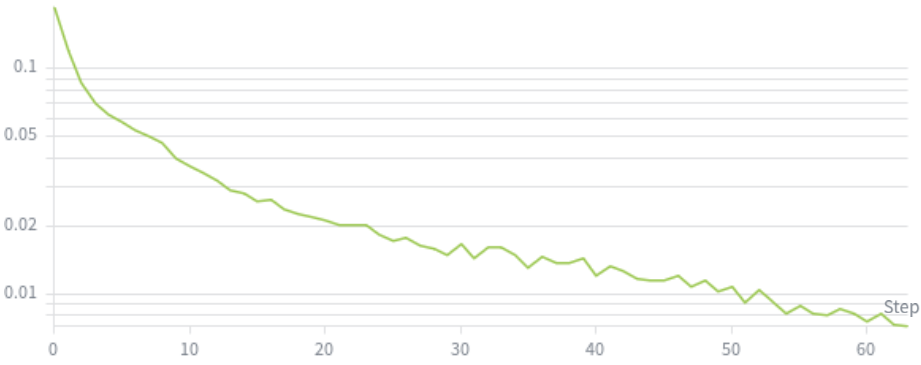
\includegraphics[height=1cm]{loss.png}
		
		% keep the main boxes roughly centered by balancing the gpu node
		\node(dummy)[above= of neuralNetwork] {};
		\node(gpu)[draw, visible on=<4>, label={[visible on=<4>]below:GPU}, below= of neuralNetwork]{\includegraphics[height=1cm]{gpu.pdf}};
	\end{tikzpicture}
\end{frame}

\begin{frame}{Machine Learning Frameworks}
	\begin{columns}
		\begin{column}{0.45\textwidth}
			\centering
			
\includegraphics[height=1cm]{pytorch-logo.png}
			PyTorch
		\begin{itemize}
			\item<2-> De facto standard for deep learning
		%	\item Primary interface is Python but also supports C++
			\item<3-> Most commonly used primitives built-in
		\end{itemize}
			\end{column}
		\begin{column}{0.45\textwidth}
			\centering
			
\includegraphics[height=1cm]{jax_logo_250px.png}
			jax
			\begin{itemize}
				\item<4-> Framework for differentiable programming
				\item<5-> Supports TPUs
				%\item Python only (C++ backend does not have user friendly API)
				%\item Extra libraries for common components
			\end{itemize}
		\end{column}
	\end{columns}
\end{frame}

\begin{frame}{Problem Description}
	\centering
	\begin{align*}
	-u''(x) &= f(x), x \in [0,1], \\
	u(0) &= u(1) = 0, \\
		f(x)=\sum_{k=1}^K a_k \sin(2\pi k x)&+b_k\cos(2\pi k x),
	\quad a_k,b_k\sim \mathcal N(0,1).
	\end{align*}
	\visible<2->{
	\begin{tikzpicture}
		\begin{axis}[%
			%xlabel=$x$,
			height=4cm,
			width=8cm,
			legend pos=south east,
			]
			\addplot table[x=x,y=f] {data/poisson.txt};
			\addplot table[x=x,y=u] {data/poisson.txt};
			\legend{$f$, $u$}
		\end{axis}
	\end{tikzpicture}
	}
\end{frame}

\begin{frame}{Artificial Neural Network I}
$\text{MLP}: \R^{N_\text{in}} \to \R^{N_\text{out}}$  with 
\[
\text{MLP}(x) := (g_L\circ\cdots\circ g_1)(x)
\] 
with layers $g_i : \R^{N_i} \to \R^{N_{i+1}}$, where
\begin{align*}
	g_1(x) &= \sigma ( W_1 x + b_1) \\
	g_j(x) &= \sigma (W_j x + b_j) + x,\quad j = 2,\dots,\,L-1\, \\
	g_L(x) &= W_L x + b_L.
\end{align*}
learned weight matrix $W_i \in \R^{N_i \times N_{i+1}}$ and bias $b_i \in \R^{N_{+1}}$
\end{frame}

\begin{frame}{Universal Approximation Theorem\footcite{Leshno1993}}
		Let $K \subseteq \R^n$ be compact. Let $\mathbf{M}$ denote the space of functions $\text{MLP}: \R^{N_\text{in}} \to \R^{N_\text{out}}$of the form 
		\[
		\text{MLP}(x) = W_2 \sigma(W_1 x + b),
		\]
		where $W \in \R^{N_\text{hid} \times N_\text{in}}, b \in \R^{N_\text{hid}}, W \in \R^{N_\text{out} \times N_\text{hid}}$ and $\sigma:\R \rightarrow \R$ is continuous. \visible<2->{Then, if and only if $\sigma$ is not a polynomial, there exists a $\text{MLP} \in \mathbf{M}$ for any continuous function $f: K \rightarrow \R$ and every $\epsilon > 0$ such that
		\[
		\sup \limits_{x \in K} ||\text{MLP}(x) - f(x)|| < \epsilon.
		\]
		}
\end{frame}

\begin{frame}{Optimizer}
	mini-batch  $(f,u)$  with $f,u \in \R^{B \times N}$
	\visible<2->{
	\[
	\mathcal{L} (u, \hat{u}) = \frac{1}{BN} \sum_{i=1}^B \sum_{j=1}^N (u_{ij} - \hat{u}_{ij})^2
	\]
 }
\visible<3->{
	\[
	w_{r+1} = w_r - \eta \frac{\partial}{\partial w}\mathcal{L}(u, \text{MLP}(f;w_r)),
	\]
	with learning rate $\eta > 0$
}
\end{frame}

\begin{frame}[fragile]{Getting Started}
	\footnotesize
	\begin{itemize}
		\item Clone repository
		\begin{minted}{bash}
git clone
		\end{minted}
		\item Create Python virtual environment
		\begin{minted}{bash}
python -m venv pytorch-env
source pytorch-env/bin/activate
		\end{minted}
		\item Install PyTorch (\url{https://pytorch.org/get-started/locally/})
		\begin{minted}{bash}
pip install torch --index-url \
https://download.pytorch.org/whl/cpu
		\end{minted}
		\item Install other Python packages
		\begin{minted}{bash}
pip install -r requirements.txt
		\end{minted}
	\end{itemize}
\end{frame}

\begin{frame}[fragile]{Regularization}
	\begin{center}
	\begin{tikzpicture}
		\begin{axis}[%
			legend pos=north west,
			%legend style={at={(0.5, 0.95)},anchor=north},
			width =0.9\textwidth,
			height=0.9\textheight,
			]
			 \addplot+[only marks] coordinates {
				(0.0, 0.2123391181230545)
				(0.10904505848884583, 0.1818249672651291)
				(0.1962873935699463, 0.18340450525283813)
				(0.2523225247859955, 0.30424225330352783)
				(0.36371058225631714, 0.5247564315795898)
				(0.42519286274909973, 0.4319450259208679)
				(0.5032525658607483, 0.29122912883758545)
				(0.6307775974273682, 0.6118528842926025)
				(0.714948296546936, 0.13949386775493622)
				(0.79041987657547, 0.29214465618133545)
				(0.8485640287399292, 0.3663618564605713)
				(0.9215502738952637, 0.4560699760913849)
				(1.0, 0.7851759791374207)
				
			}; 
			
			\addplot+[no markers, thick, visible on=<2->] table[x index=0, y index=1,] {data.txt};
			\addplot+[no markers, thick, visible on=<3->] table[x index=0, y index=1] {data_small.txt};
			\addplot+[no markers, thick, visible on=<4->] table[x index=0, y index=1] {data_wd.txt};
			
			\only<1>{\legend{samples, ,,}}
			\only<2>{\legend{samples, NN,,}}
			\only<3>{\legend{samples, NN, small NN, }}
			\only<4>{\legend{samples, NN, small NN,  NN+weight decay}}
		\end{axis}
	\end{tikzpicture}
	\end{center}
\end{frame}

\begin{frame}{Regularization Techniques}
	Weight decay (Tikhonov regularization)
	\[
	\hat{\mathcal{L}} (u, \hat{u}, w_r) = \mathcal{L} (u,\hat{u}) + \lambda ||w_r||^2
	\]
	\visible<2->{
	Layer normalization
	\[
	\text{LN}(x) = \frac{x - \text{E}[x]}{\text{Var}[x]} \odot \gamma + \beta
	\]
	}
\end{frame}

\begin{frame}{Further Reading}
	\begin{itemize}
		\item Intuitive explanation of generalization abilities of SGD \\
		{\footnotesize
			\fullcite{Huang2019}
		}
		\item AdamW and weight decay \\
		{\footnotesize
			\fullcite{Loshchilov2017}
		}
		\item Normalization techniques \\
		{\footnotesize
			\fullcite{Huang2023}
		}
	\end{itemize}
\end{frame}

\end{document}
